% План на главу
% 0) Фотонное излучение от радионуклидов
% 1) Описать про датчики в системе аскро и их характеристики (дальность, макс мощность и тд)
% 2) Описать, зачем в модели аскро нужны датчики
% 3) Описать формулу для расчета
% 4) Описать реализацию непосредственно в коде
% ПРОВЕРИТЬ НА ОРФОГРАФИЮ!!

\chapter{Разработка модуля расчета мощности дозы внешнего гамма-излучения}
\label{chapter_dose}

\section{Необходимость расчета мощности дозы гамма-излучения}

Радиоактивные нуклиды, которые могут попасть в атмосферу в результате аварии на \ac{aes}, являются бета-активными. При 
протекании бета-распада результирующее ядро может оказаться в возбужденном состоянии. Возбуждение ядра снимается 
посредством испускания гамма-квантов. Для примера, на рисунке \ref{fig_I_133_decay_gamma} представлена упрощенная схема 
распада изотопа $^{131}I$, после которого образуется изотоп $^{131}Xe$ в возбужденном состоянии, испускающий 
гамма-кванты при переходе в основное состояние.

\begin{figure}[ht!]
    \centering
    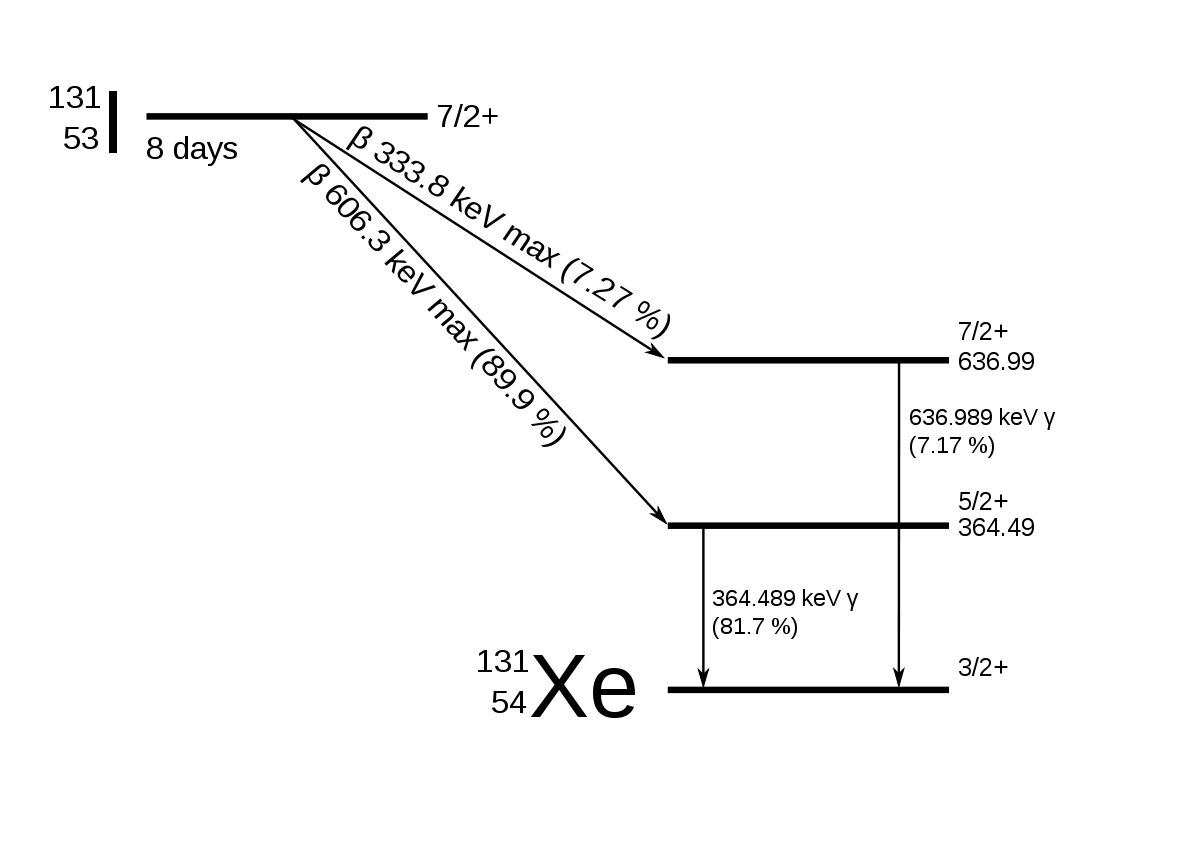
\includegraphics[width=13cm]{I_133_decay_gamma}
    \captionsetup{justification=centering}
    \caption{Упрощенная схема распада изотопа $^{131}I$.}
    \label{fig_I_133_decay_gamma}
\end{figure}

Одной из главных задач современных систем \ac{ascro} на \ac{aes} является измерение значений мощности дозы 
гамма-излучения на прилегающей к \ac{aes} местности. Значение мощности дозы гамма-излучения на местности необходимо знать 
для контроля радиационной обстановки вокруг \ac{aes}, а также своевременной выдаче рекомендаций по принятию решений о 
защите населения. Измерение мощности дозы гамма-излучения в системах \ac{ascro} проводится при помощи 
специализированных датчиков радиационного контроля, расположенных на прилегающей к \ac{aes} местности. 

\section{Датчики радиационного контроля}

Основу \ac{ascro} составляет система постов радиационного контроля гамма-излучения, расположенных вокруг \ac{aes}. 
Обычно, измерительные блоки фотонного излучения содержат датчики двух диапазонов: $10^{-7}$ - $10^{-3}$ Зв и $10^{-3}$ 
- $10$ Зв. В качестве блоков детектирования в системах постов радиационного контроля \ac{ascro} используются БДМГ-08Р3, 
БДМГ-08Р4, БДМГ-08Р5, БДМГ-100 \cite{elokhin}. Для примера, рассмотрим технические характеристики блока детектирования 
БДМГ-100.

Блок детектирования БДМГ-100 предназначен для непрерывного измерения \ac{maed} (\acl{maed}) \cite{bdmg-100}. Блок 
применяется для контроля радиационной обстановки на объектах атомной энергетики и радиохимического производства; на 
промышленных предприятиях, использующих источники ионизирующих излучений; на пунктах специального и таможенного контроля 
и в службах экологического и санитарно-эпидемиологического надзора. В таблице \ref{table_bdmg_100} приведены основные 
техническите характеристики блока детектирования БДМГ-100.

\begin{table}[ht]
	\setlength{\extrarowheight}{1mm} 
	\caption{Основные технические характеристики блока детектирования БДМГ-100 \cite{bdmg-100}.}
	\label{table_bdmg_100}
	\centering
    \begin{tabular}{|M{0.6\textwidth}|M{0.3\textwidth}|}
    \hline Характеристика & Значение \\
    \hline Диапазон энергий регистрируемого гамма-излучения & от 0,05 до 3,0 МэВ \\
    \hline Диапазон измерений МАЭД гамма-излучения в чувствительном поддиапазоне & от 0,1 мкЗв/ч до 2 мЗв/ч \\
    \hline Диапазон измерений МАЭД гамма-излучения в грубом поддиапазоне & от 0,5 мЗв/ч до 10 Зв/ч \\
    \hline Пределы допускаемой основной относительной погрешности измерений МАЭД гамма-излучения & $\pm$(15 + 3/Н*) \% \\
    \hline Время установления рабочего режима блока & не превышает 1 мин \\
    \hline Время непрерывной работы & не ограничено \\
    \hline Напряжение питания постоянного тока & 12 $\pm$ 0,5 В \\
    \hline \makecell{Потребляемый ток при напряжении \\ питания 12 В} & не более 25 мА \\
    \hline Температура окружающего воздуха & от -40 до +50 °С \\
    \hline Относительная влажность окружающего воздуха & до 98 \% при +35 °С \\
    \hline Атмосферное давление & от 84,0 до 106,7 кПа \\
    \hline 
    \end{tabular}
\end{table}

Принцип работы блока БДМГ-100 основан на преобразовании энергии ионизирующих излучений в электрические импульсы. В 
качестве детекторов ионизирующего излучения в блоках БДМГ-100 используются газоразрядные счетчики Гейгера-Мюллера, а 
именно: для чувствительного поддиапазона 2 счетчика СБМ20, а для грубого поддиапазона один счетчик Гамма-1 (СИ-34Г). На 
рисунке \ref{fig_bdmg_100} представлены габаритные и присоединительные размеры блока БДМГ-100.

\begin{figure}[ht!]
    \centering
    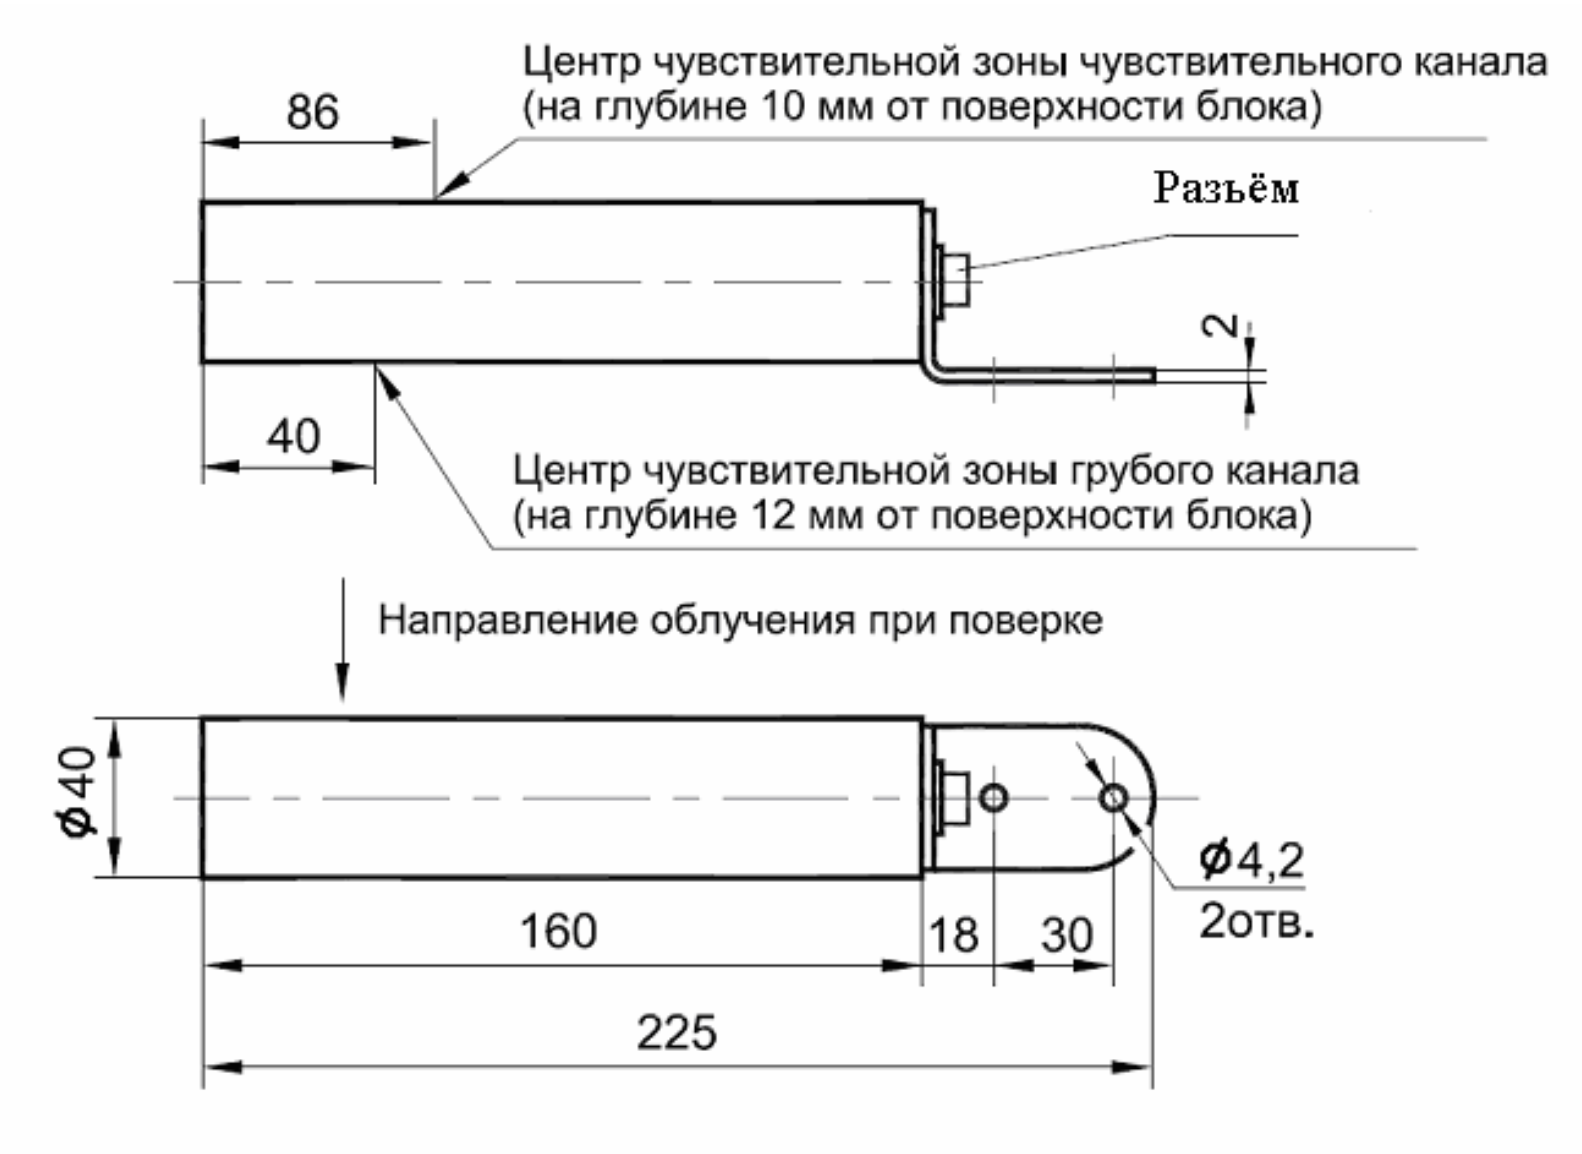
\includegraphics[width=13cm]{bdmg-100}
    \captionsetup{justification=centering}
    \caption{Габаритные и присоединительные размеры блока БДМГ-100 \cite{bdmg-100}.}
    \label{fig_bdmg_s100}
\end{figure}

Измерение мощности дозы гамма-излучения в системах \ac{ascro} выполняется при помощи датчиков радиационного контроля, 
размещенных вокруг \ac{aes}. Одной из важнейших задач проектирования систем \ac{ascro} является их оптимизация. Под 
оптимизацией \ac{ascro} понимается выбор необходимого и достаточного количества датчиков радиационного контроля, 
размещенных вокруг \ac{aes}, а также методы их размещения, при помощи которых можно повысить точность прогностических 
расчетов при оценке уровней радиационного загрязнения подстилающей поверхности, дозовых нагрузок на персонал и население 
в случае радиационной аварии.

\section{Оптимизация количества датчиков радиационного контроля}

При проектировании систем \ac{ascro} ставится задача обеспечения наибольшей точности измерений и контроля радиационного 
загрязнения внешней среды. 

Основным средством измерения \ac{ascro} являются гамма-датчики, которые требуют для нормальной работы основные и 
дополнительные линии связи электрического питания, автономного питания и другого оборудования, стоимость которых 
определяет главные затраты на систему. С другой стороны, увеличение числа датчиков радиационного контроля повышает 
надежность и достоверность информации о зоне и уровне загрязнения внешней среды. Таким образом, ставится задача 
оптимизации числа датчиков радиационного контроля с экономической (уменьшение затрат на систему) и экологической 
(повышение точности измерений) точек зрения.

В таблице \ref{table_aes_ascro} приведено количество постов радиационного контроля на российских \ac{aes}. Из таблицы 
видно, что количество постов радиационного контроля на различных \ac{aes} различается. Кроме того, в каждом из случаев 
количество постов научно необоснованно с точки зреня оптимальности, описанной выше. Это связанно с недостаточным 
финансированием по федеральной программе «Ядерная и радиационная безопасность России» на создание \ac{ascro} 
\cite{elokhin}.

\begin{table}[ht]
	\setlength{\extrarowheight}{1mm} 
	\caption{Количество постов радиационного контроля на российских \ac{aes} \cite{elokhin}.}
	\label{table_aes_ascro}
	\centering
    \begin{tabular}{|M{0.3\textwidth}|M{0.3\textwidth}|}
    \hline \ac{aes} & Кол-во постов контроля \\
    \hline Балаковская & 25 \\
    \hline Белоярская & 8 \\
    \hline Билибинская & 10 \\
    \hline Калининская & 18 \\
    \hline Кольская & 20 \\
    \hline Курская & 29 \\
    \hline Ленинградская & 14 \\
    \hline Нововоронежская & 22 \\
    \hline Ростовская & 19 \\
    \hline Смоленская & 18 \\
    \hline 
    \end{tabular}
\end{table}